%%%%%%%%%%%%%%%%%%%%%%%%%%%%%%%%%%%%%%%%%%%%%%%%%%%%%%%%%%%%%%%%%%%%%%%%%%%%%%%%%%%%
%Do not alter this block of commands.  If you're proficient at LaTeX, you may include additional packages, create macros, etc. immediately below this block of commands, but make sure to NOT alter the header, margin, and comment settings here. 
\documentclass[12pt]{article}
\usepackage[margin=1in, bottom=4.5cm]{geometry}
\usepackage{amsmath,amsthm,amssymb,amsfonts, enumitem, fancyhdr, color, comment, graphicx, environ, scrextend, mathtools, yfonts, pdfpages}
\usepackage[table,dvipsnames]{xcolor}
\usepackage{tikz}  
\usepackage{tikz-3dplot} 
\usepackage{amssymb}
\usepackage{xifthen}
\pagestyle{fancy}
\setlength{\headheight}{65pt}
\newenvironment{problem}[2][Problem]{\begin{trivlist}
\item[\hskip \labelsep {\bfseries #1}\hskip \labelsep {\bfseries
#2.}]}{\end{trivlist}}
\newenvironment{lemma}[2][Lemma]{\begin{trivlist}
\item[\hskip \labelsep {\bfseries #1}\hskip \labelsep {\bfseries #2.}]}{\end{trivlist}}
\newenvironment{theorem}[2][Theorem]{\begin{trivlist}
\item[\hskip \labelsep {\bfseries #1}\hskip \labelsep {\bfseries #2.}]}{\end{trivlist}} 
\newenvironment{sol}
    {\emph{Proof.}
    }
    {
    \qed
    }
\specialcomment{com}{ \color{blue} \textbf{Comment:} }{\color{black}} %for instructor comments while grading
\NewEnviron{probscore}{\marginpar{ \color{blue} \tiny Problem Score: \BODY \color{black} }}
%%%%%%%%%%%%%%%%%%%%%%%%%%%%%%%%%%%%%%%%%%%%%%%%%%%%%%%%%%%%%%%%%%%%%%%%%%%%%%%%%

\newcommand\restr[2]{{% we make the whole thing an ordinary symbol
  \left.\kern-\nulldelimiterspace % automatically resize the bar with \right
  #1 % the function
  \vphantom{\big|} % pretend it's a little taller at normal size
  \right|_{#2} % this is the delimiter
  }}





%%%%%%%%%%%%%%%%%%%%%%%%%%%%%%%%%%%%%%%%%%%%%
%Fill in the appropriate information below
\lhead{Trey Manuszak}  %replace with your name
\rhead{MAT 473: Intermediate Real Analysis II \\ Final} %replace XYZ with the homework course number, semester (e.g. ``Spring 2019"), and assignment number.
%%%%%%%%%%%%%%%%%%%%%%%%%%%%%%%%%%%%%%%%%%%%%

\usepackage{blindtext}
\title{MAT 473: Intermediate Real Analysis II}
\date{May 8, 2020}
\author{Trey Manuszak\\ Arizona State University}


%%%%%%%%%%%%%%%%%%%%%%%%%%%%%%%%%%%%%%
%Do not alter this block.
\begin{document}
%%%%%%%%%%%%%%%%%%%%%%%%%%%%%%%%%%%%%%
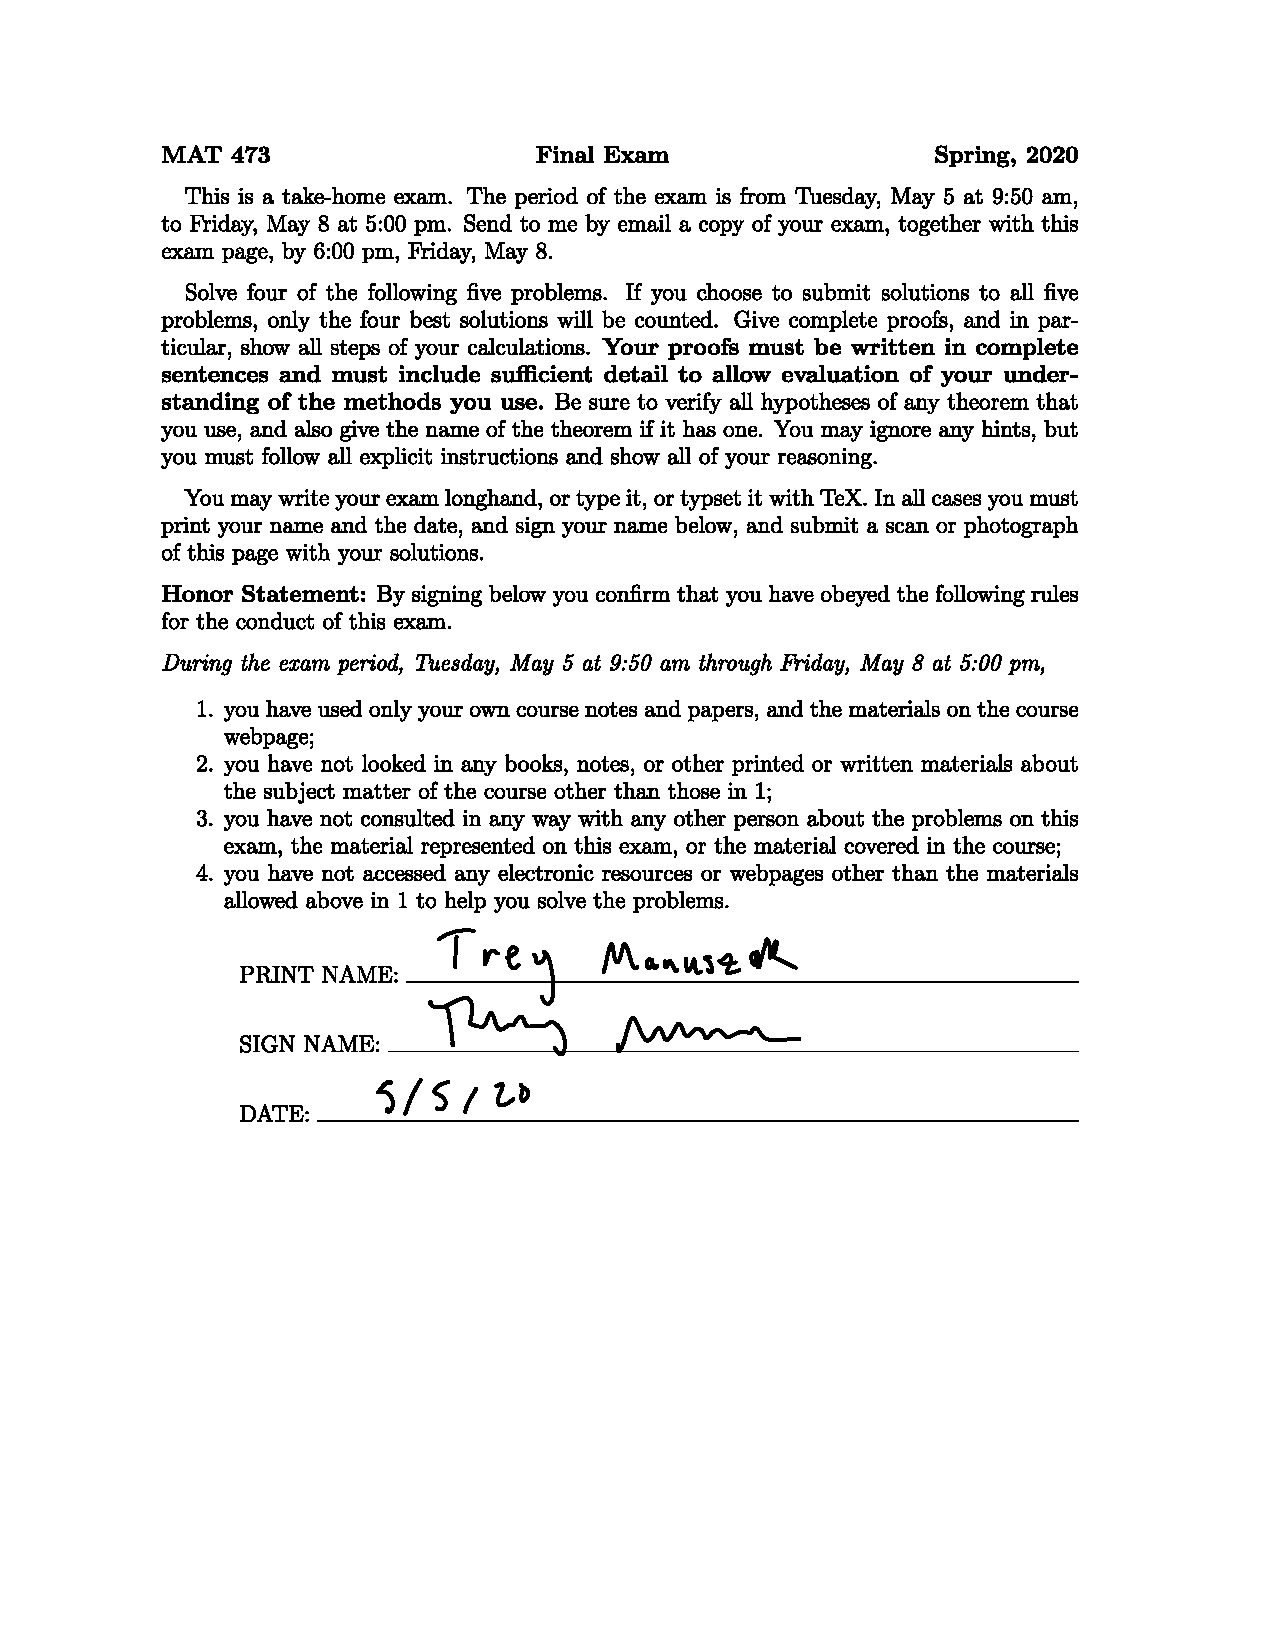
\includepdf[page={1}]{473finalpg1.pdf}

\maketitle
\newpage


%Copy the following block of text for each problem in the assignment.
\begin{problem}{1}
Let $U \subseteq \mathbb{R}^{3}$ be an open set, let $f : U \to \mathbb{R}$ be continuously differentiable, and let $p = (x_0, y_0, z_0) \in U$ and $c = f(p)$. We let $(x,y,z)$ denote the coordinates in $\mathbb{R}^3$. Using the implicit function theorem, and the equation $f(x,y,z) = c$, we can give a precise meaning to the classical expression $\frac{\partial y}{\partial x}$.
\begin{itemize}
  \item[(a)] What is this meaning? Explain carefully.
  
  \hspace{1em} In physical terms, we would be able to find a directional derivative, or quantify a change in direction $y$ for a certain change in direction $x$. Given an example of a surface where this is not always possible, if you consider a function which goes through the cartesian point $(1,0,0) \in S$ with $S$ being a unit sphere. Then, there does not exist a function that can represent $y$ in terms of $x$ and $z$ on the function $f$, since $\frac{\partial y}{\partial x}$ would be undefined for any function going through that point on the surface of the unit sphere. 

  \item[(b)] What condition guarantees that $\frac{\partial y}{\partial x}$ makes sense?
  
  \hspace{1em} Since we can supposedly find $\frac{\partial y}{\partial x}$, then we must've found a function, which approximates $y$ defined as $y : B_s(x_0,z_0) \to B_r(y_0)$, which approximates the level set $\{(x,y,z) \in U : f(x,y,z) = c\}$ such that $f(x,y(x,z),z) = c$ for some $s,r > 0$. This function $y$ is continuously differentiable and if $f(x,y(x,z),z) = c$ is differentiated with respect to $x$, will yield $$f_x + f_y \cdot \frac{\partial y}{\partial x} + f_z \cdot 0 = 0.$$ We can then solve $\frac{\partial y}{\partial x} = -\frac{f_x}{f_y}$. So, since $\frac{\partial y}{\partial x}$ exists, $f_y$ must be invertible, or not equal to zero. Also, since the function $y$ represented in terms of $x$ and $z$ exist, we must have used implicit function theorem, which relies on $p \in U$ open with $f$ being continuously differentiable and $f(p) = c$.
  
  \item[(c)] Prove the "paradox of classical notation": $\frac{\partial y}{\partial x} \cdot \frac{\partial z}{\partial y} \cdot \frac{\partial x}{\partial z} = -1$. State the result as a precise theorem (in non-classical notation), and be sure to give the necessary hypothesis.  
  
  \begin{theorem}{1}
    Let $U \subseteq \mathbb{R}^{3}$ be an open set, let $f : U \to \mathbb{R}$ be continuously differentiable, and let $p = (x_0, y_0, z_0) \in U$ and $c = f(p)$. Suppose there is a continuously differentiable function $y : B_s(x_0,z_0) \to B_r(y_0)$ such that $f(x,y(x,z),z) = c$ and $f_y \neq 0$. Suppose there is a continuously differentiable function $z : B_u(x_0,y_0) \to B_t(z_0)$ such that $f(x,y,z(x,y)) = c$ and $f_z \neq 0$. Suppose there is a continuously differentiable function $x : B_w(y_0,z_0) \to B_v(x_0)$ such that $f(x(y,z),y,z) = c$ and $f_x \neq 0$. Then $\frac{\partial y}{\partial x} \cdot \frac{\partial z}{\partial y} \cdot \frac{\partial x}{\partial z} = -1$.
  \end{theorem}

  \begin{sol}
    By applying the implicit function theorem in three different instances, we can show that $\frac{\partial y}{\partial x} = -\frac{f_x}{f_y}$, $\frac{\partial z}{\partial y} = -\frac{f_y}{f_z}$, and $\frac{\partial x}{\partial z} = -\frac{f_z}{f_x}$. Thus, \begin{align*}
      \frac{\partial y}{\partial x} \cdot \frac{\partial z}{\partial y} \cdot \frac{\partial x}{\partial z} &= \left( -\frac{f_x}{f_y} \right) \left( -\frac{f_y}{f_z} \right) \left( -\frac{f_z}{f_x} \right) \\ &= -1.
    \end{align*}
  \end{sol}

  \hspace{1 em} The real problem that I see with the classical notation is that $\frac{\partial y}{\partial x}$ appears to be a fraction (which it is!) but it is hard to see domain restrictions as $\partial x$ alone does not represent anything, hence why it looks like everything should "paradoxically" cancel to be 1, but doesn't.
\end{itemize}
\end{problem}

\begin{problem}{2}
Let $U \subseteq \mathbb{R}^2$ be an open connected set and let $f : U \to \mathbb{R}$ be continuously differentiable. Suppose that $\frac{\partial f}{\partial y} = 0$ throughout $U$.
\begin{itemize}
  \item[(a)] Suppose that $U$ has the following property: for every vertical line $L \subseteq \mathbb{R}^2$, the intersection $U \cap L$ is a subinterval of $L$. Prove that for all $x, y_1, y_2$ such that $(x,y_1)\in U$ and $(x,y_2) \in U$, we have $f(x,y_1) = f(x,y_2)$ (we say that $f$ is \textit{independent of y}).
  
  \begin{sol}
    Let $U \subseteq \mathbb{R}^2$ be an open connected set and let $f : U \to \mathbb{R}$ be continuously differentiable. Suppose that $\frac{\partial f}{\partial y} = 0$ throughout $U$. Let $L = \{(x,y) \in \mathbb{R}^2 : x \text{ is fixed}\} \subseteq U$. Then, since $f$ is differentiable and $L$ is convex, by the mean value theorem, for $\overline{ab} \subseteq L$, there exists $c \in \overline{ab}$ such that $f(b) - f(a) = f'(c)(b-a)$. But, $f'(c) = 0$ by hypothesis. Thus, $f(a) = f(b)$, which implies for $(x,y_1),(x,y_2) \in U$, $f(x,y_1) = f(x,y_2)$.
  \end{sol}

  \item[(b)] Let $U = \mathbb{R}^2 \setminus ((-\infty,0] \times \{0\})$. (Thus $U$ equals the plane with the nonpositive x-axis removed.) Find a counterexample to the result in part (a)  for $U$, and prove that your counterexample does the job. (In other words find a continuously differentiable function $f : U \to \mathbb{R}$ such that $\frac{\partial f}{\partial y} = 0$ throughout $U$, but such that there exist $x,y_1,y_2$ such that $(x,y_1),(x,y_2) \in U$ and $f(x,y_1) \neq f(x,y_2)$ - and prove that your function $f$ does have all of these properties.)
  
  \begin{sol}
    Let $U = \mathbb{R}^2 \setminus ((-\infty,0] \times \{0\})$ and $f : U \to \mathbb{R}$ be defined by $$f(x,y) = \begin{cases} 
      x^2 & \text{if } x,y < 0 \\
      0 & \text{else}
   \end{cases}$$
   Then, we have that $f_y = 0$ throughout $U$, and $f_x = 2x$, which is continuous over $U$. However, $f(1,1) = 1$, but $f(1,-1) = 0$. Thus, there exists a continuously differentiable function $f : U \to \mathbb{R}$ such that $\frac{\partial f}{\partial y} = 0$ throughout $U$, and there exists $(x,y_1),(x,y_2) \in U$ with $f(x,y_1) \neq f(x,y_2)$.
  \end{sol}
\end{itemize}
\end{problem}

\begin{problem}{3}
Let $f : \mathbb{R} \to \mathbb{R}$ be Lipschitz, and let $E \subseteq \mathbb{R}$ be a measurable set with $m(E) = 0$. Prove that $m(f(E)) = 0$. (Hint: write open intervals in the form $(a - r, a + r)$ rather than in the form $(a,b)$.) (Recall that $f$ is \textit{Lipschitz} if there is a constant $C > 0$ such that for all $x,y \in \mathbb{R}$, $\left| f(x) - f(y) \right| \leq C \left| x - y \right|$.)
\end{problem}

\begin{sol}
  Let $f : \mathbb{R} \to \mathbb{R}$ be $C$-Lipschitz, with $C > 0$, and let $E \subseteq \mathbb{R}$ be a measurable set with $m(E) = 0$. Since $E$ has measure zero, for $\epsilon > 0$ arbitrary but fixed, there exists open intervals $A_n = (a - r_n, a + r_n)$, such that it creates a countable open cover, $E \subseteq \cup_{n \in \mathbb{N}}A_n$, and $m(E) \leq \sum_{n \in \mathbb{N}}m(A_n) < \epsilon$. Looking at each $n$, we have the following
  \begin{align*}
    m(f(A_n)) &= \left| f(a-r_n) - f(a+r_n) \right| \tag*{(By Lebesgue measure on $\mathbb{R}$)}\\
    &\leq C \cdot \left| a - r_n - (a + r_n) \right| \tag*{(Since $f$ is $C$-Lipschitz)} \\
    &= C \cdot \left| A_n \right|. 
  \end{align*}
  Now, we get
  \begin{align*}
    m(f(E)) &\leq m\left( f \left( \bigcup_{n \in \mathbb{N}}A_n \right) \right) \tag*{(By monotonicity)} \\
    &= m \left( \bigcup_{n \in \mathbb{N}} f(A_n) \right) \tag*{(By continuity of $f$)} \\
    &\leq \sum_{n \in \mathbb{N}} m(f(A_n)) \tag*{(By subadditivity and $C$-Lipschitz property of $f$)} \\
    &< C \cdot \epsilon.
  \end{align*}
  \hspace{1em} Therefore, since epsilon was arbitrary, we can conclude $m(f(E)) = 0$.
\end{sol}

\begin{problem}{4}
Let $f : \mathbb{R} \to \mathbb{R}$ be a nonnegative measurable function. Suppose that $\int f = 0$. Prove that $f = 0$ almost everywhere. (Hints: let $E_n = \{f \geq \frac{1}{n}\}$ and let $p_n = \frac{1}{n} \chi_{E_n}$.)
\end{problem}

\begin{sol}
  Suppose for some $X \subseteq \text{dom}(f)$ that is measurable, $\int_X f = 0$. Let $E_n = \{x \in X : f(x) > \frac{1}{n}\}$. Then, $\{x \in X : f(x) > 0\} = \cup_{n \in \mathbb{N}}E_n$. Then, 
          \begin{align*}
            m(E_n) &= \int_{E_n}1 \cdot \chi_{E_n} \\
            &= n \int_{E_n} \frac{1}{n} \cdot \chi_{E_n} \\
            &\leq n \int_{E_n} f \\
            &\leq n \int_{X} f \\
            &=0.
          \end{align*}
          Therefore, $m(E_n) = 0$, which implies $f = 0$ a.e., since $X$ was an arbitrary measurable set in the domain of $f$ and $\{x \in X : f(x) > 0\} = \cup_{n \in \mathbb{N}}E_n$.
\end{sol}

\begin{problem}{5}
For $n = 1,2,3,\dots$ let $f_n : \mathbb{R} \to \mathbb{R}$ be a nonnegative measurable function. Suppose that the sequence $(f_n)$ is decreasing, in the sense that for each $x \in \mathbb{R}$, $f_1(x) \geq f_2(x) \geq f_3(x) \geq \dots$. Suppose further that $\lim_{n \to \infty} \int f_n = 0$. Prove that $(f_n) \to 0$ almost everywhere.
\end{problem}

\begin{sol}
  For $n = 1,2,3,\dots$ let $f_n : \mathbb{R} \to \mathbb{R}$ be a nonnegative measurable function. Suppose that the sequence $(f_n)$ is decreasing, in the sense that for each $x \in \mathbb{R}$, $f_1(x) \geq f_2(x) \geq f_3(x) \geq \dots$. Suppose further that $\lim_{n \to \infty} \int f_n = 0$. Since each $f_n$ is nonnegative measurable and pointwise decreasing as $n \to \infty$, then $(f_n) \to f$ pointwise for some $f$. By letting $g = f_1$, by Lebesgue's dominated convergence theorem, we know that $\int f = \lim_{n \to \infty} \int f_n$. Since $\lim_{n \to \infty} \int f_n = 0$ by assumption, then $\int f = 0$. By Exercise 21.6 (2), we know that since $\int f = 0$, then $f = 0$ almost everywhere. Therefore, since $\lim_{n \to \infty} f_n = f$, then $\lim_{n \to \infty} f_n \to 0$ almost everywhere, transitively.
\end{sol}
%%%%%%%%%%%%%%%%%%%%%%%%%%%%%%%%%%%%%%%%
%Do not alter anything below this line.
\end{document}